% "Станет проще"

\documentclass[a4paper,12pt]{article} % тип документа

% report, book

% Рисунки
\usepackage{graphicx}
\usepackage{wrapfig}

\usepackage{hyperref}
\usepackage[rgb]{xcolor}



%  Русский язык

\usepackage[T2A]{fontenc}			% кодировка
\usepackage[utf8]{inputenc}			% кодировка исходного текста
\usepackage[english,russian]{babel}	% локализация и переносы


% Математика
\usepackage{amsmath,amsfonts,amssymb,amsthm,mathtools} 


\usepackage{wasysym}

%Заговолок
\author{Сафиуллин Роберт	}
\title{Лабораторная работа 2.1.4}
\date{\today}





\begin{document} % начало документа

\maketitle


\newpage
\section{Цель работы:}
1) измерение количества подведенного тепла и вызванного им нагрева твердого тела; 2)определение теплоемкости по экстраполяции отношения  $\triangle Q / \triangle T$ к нулевым потерям тепла.\\
\section{В работе используются:}
 калориметр с нагревателем и термометром сопротивления; амперметр; вольтметр; мост постоянного тока; источник питания 36 В.
 \section*{Описание работы}\
\indent В предлагаемой работе измерение теплоемкости твердых тел про- изводится по обычной схеме. Исследуемое тело помещается в кало- риметр. Измеряется $\Delta Q$ — количество тепла, подведенного к телу, и $\Delta T$ — изменение температуры тела, произошедшее в результате подвода тепла. Теплоемкость определяется по формуле\\
$$C=\frac{\Delta Q}{\Delta T}=\frac{P\Delta t - \lambda (T-T_k)\Delta t}{\Delta T}=\frac{P - \lambda (T-T_k)}{\Delta T/\Delta t}$$
\ \\
$\frac{\Delta T}{\Delta t}=f(T)$ -строим график и проводим касательную при $T=T_k$\\
\ \\
Тогда $C=\frac{P}{(\Delta T/\Delta t)_k}$\\
Дополнительно $R_t=R_o(1+\alpha\Delta T)$; $\frac{dR}{dt}=R_o\alpha\frac{dT}{dt}$\\
$$C=\frac{PR_k\alpha}{(dR/dt)_k(1+\alpha\Delta T_k)}$$
\ \\
\newpage
\section{Экспериментальная установка:}
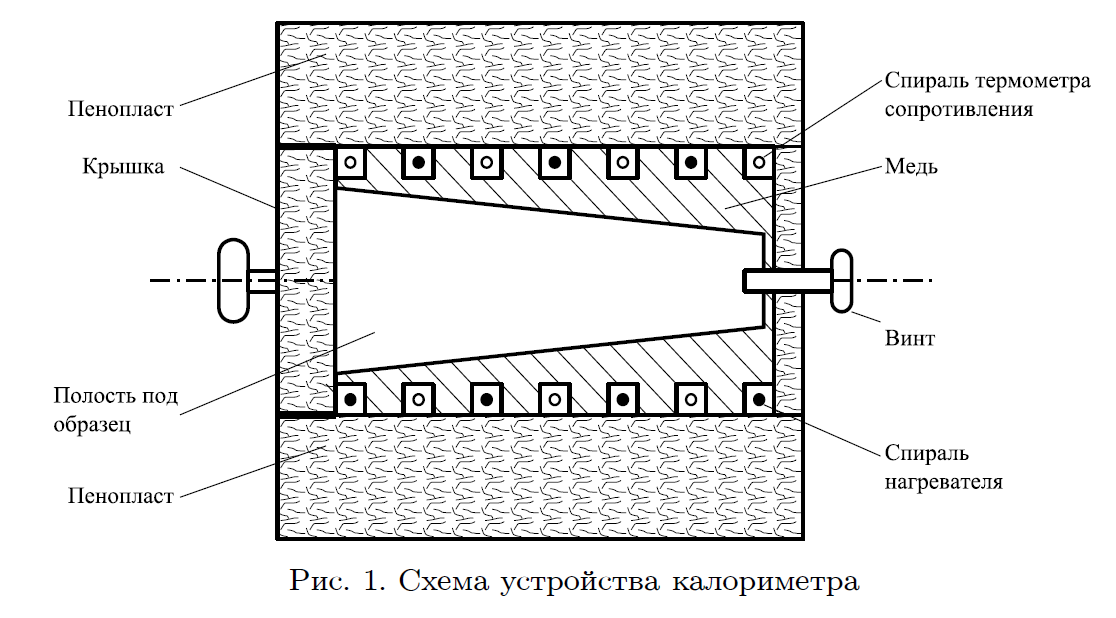
\includegraphics[scale=0.7]{ust}
\section{Ход работы}
1) Подготовим мост постоянного тока и определим R при комнатной температуре:

\textit{R}= 18.04$\Omega$

$T_k$= $28^{\circ}$C

$\alpha$ = 4.28*$10^{-3} K^{-1}$

$R_0$= 18.5$\Omega$

$P=10.8 Вт$

2) Включим источник тока и снимем зависимость сопротивления термометра от времени для пустого калориметра, а также с латунью и алюминием внутри. Для этого проверим балансировку моста и установим на нем сопротивление, немного большее ($\sim$0.5\%) чем это необходимо для балансировки.

3) Показания запишем в таблицы:


\begin{tabular}{|c|c|}
\hline
\multicolumn{2}{|c|}{Пустой калориметр} \\
\hline 
R, $\Omega$ & t, c \\ 
\hline
18.37 & 0 \\
\hline 
18.46 & 69 \\ 
\hline 
18.68 & 245 \\ 
\hline 
18.77 & 330 \\ 
\hline 
18.86 & 452 \\ 
\hline 
18.95 & 551 \\ 
\hline 
19.04 & 674 \\ 
\hline 
19.14 & 810 \\ 
\hline 
19.24 & 943 \\ 
\hline 
19.34 & 1092 \\ 

\hline 
\end{tabular} 
\begin{tabular}{|c|c|}
\hline
\multicolumn{2}{|c|}{Латунь      } \\
\hline
R, $\Omega$ & t, c \\ 
\hline 
18.65 & 0 \\ 
\hline 
18.74 & 53 \\ 
\hline 
18.83 & 187 \\ 
\hline 
18.92 & 350 \\ 
\hline 
19.01 & 497 \\ 
\hline 
19.11 & 673 \\ 
\hline 
19.21 & 864 \\ 
\hline 
19.31 & 1108 \\ 

\hline 
\end{tabular} 
\begin{tabular}{|c|c|}
\hline
\multicolumn{2}{|c|}{Алюминий      } \\
\hline
R, $\Omega$ & t, c \\ 
\hline 
18.53 & 0 \\ 
\hline 
18.62 & 114 \\ 
\hline 
18.71 & 210 \\ 
\hline 
18.80 & 354 \\ 
\hline 
18.89 & 471 \\ 
\hline 
18.98 & 636 \\ 
\hline 
19.07 & 807 \\ 
\hline 
19.17 & 955 \\ 
\hline 
19.27 & 1159 \\ 
\hline 
19.36 & 1316 \\ 
\hline 
19.46 & 1566 \\ 
\hline 
\end{tabular} 

3) Построим графики по данным таблицам:\\[0.2cm]
\begin{center}
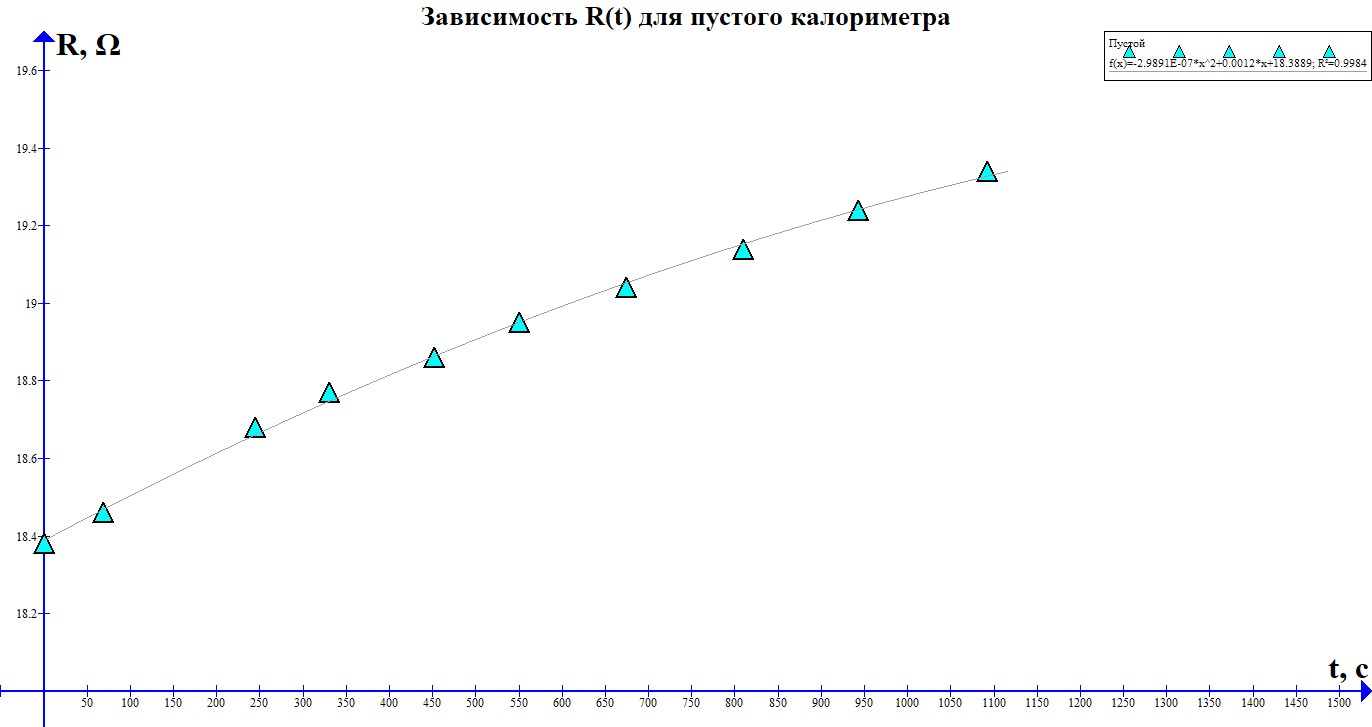
\includegraphics[scale=0.35]{2141}
\end{center}
\newpage
\begin{center}
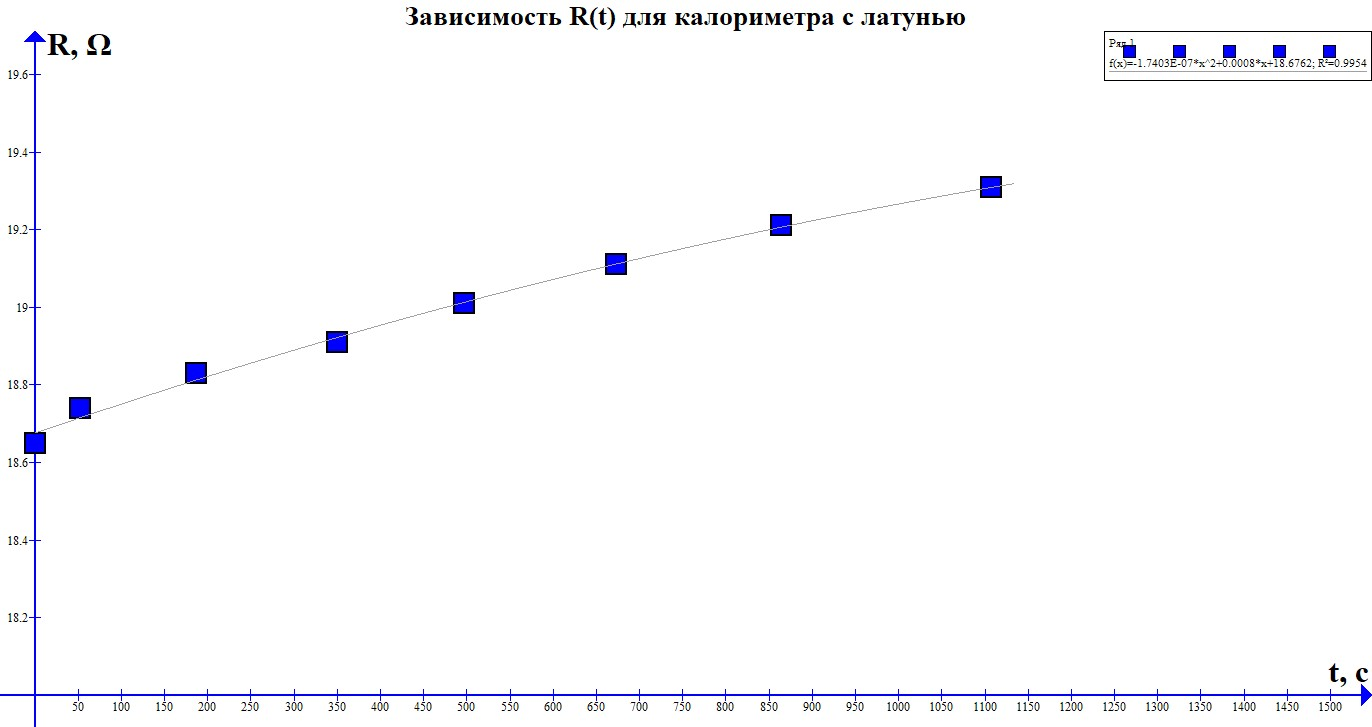
\includegraphics[scale=0.35]{2142}
\end{center}
\begin{center}
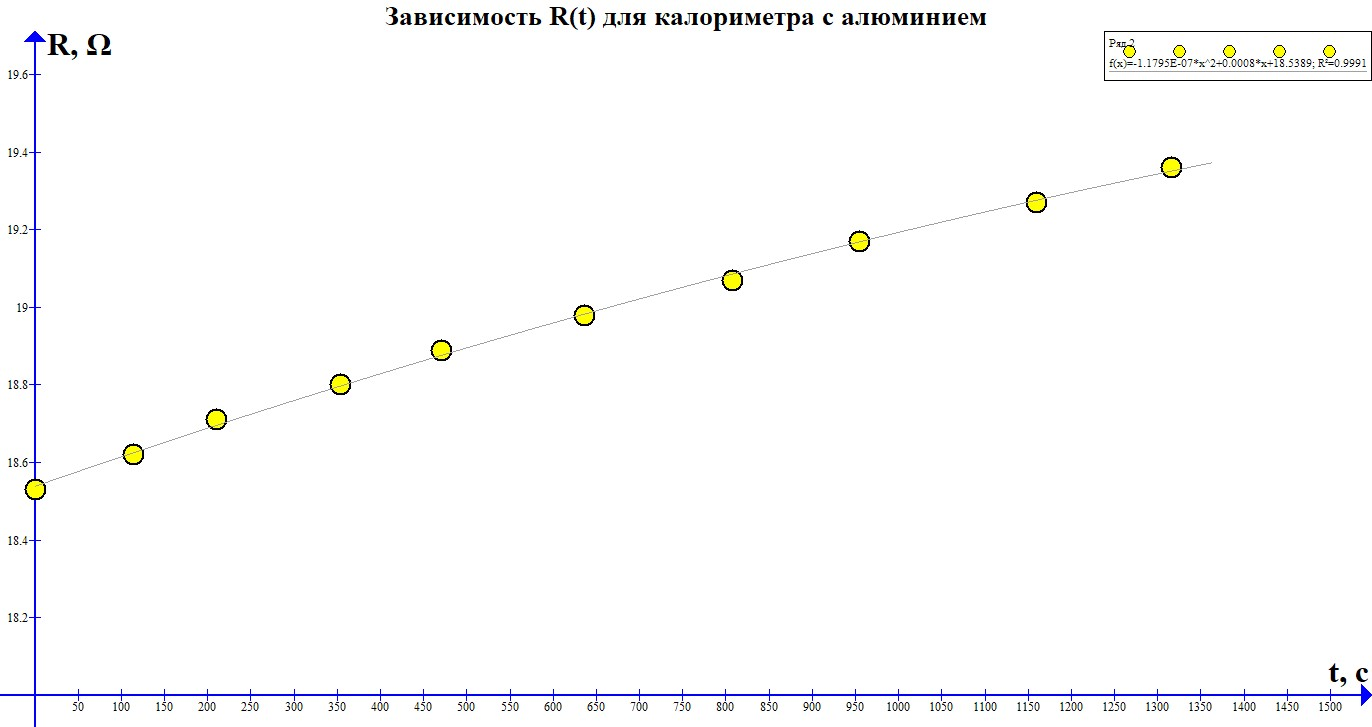
\includegraphics[scale=0.35]{2143}
\end{center}
\newpage
4) Используя полученные зависимости, построим графики зависимости $\frac{\triangle R} {\triangle t}$ от R

5) Для этого разделим кривые на отрезки и найдем для каждого из них коэффицент наклона. 

Получили:\\[0.2cm]
\begin{center}
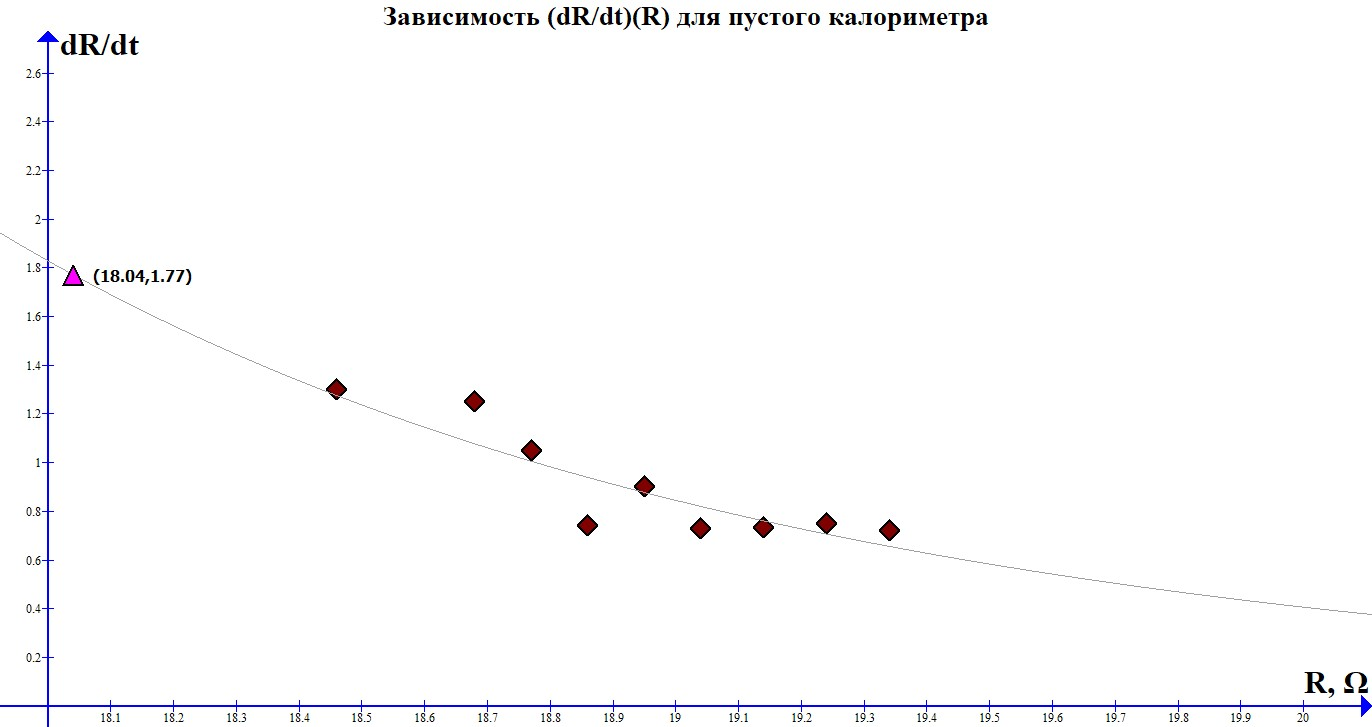
\includegraphics[scale=0.35]{2144}
\end{center}
\begin{center}
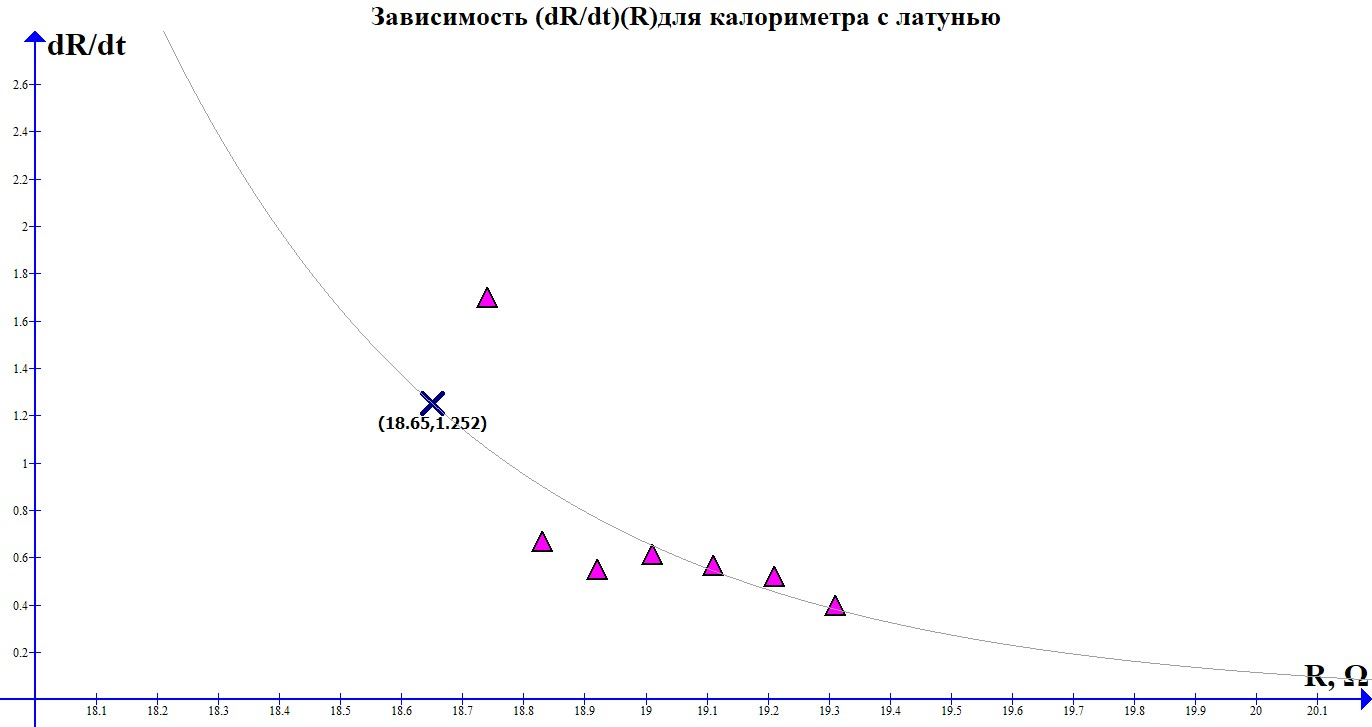
\includegraphics[scale=0.35]{2145}
\end{center}
\begin{center}
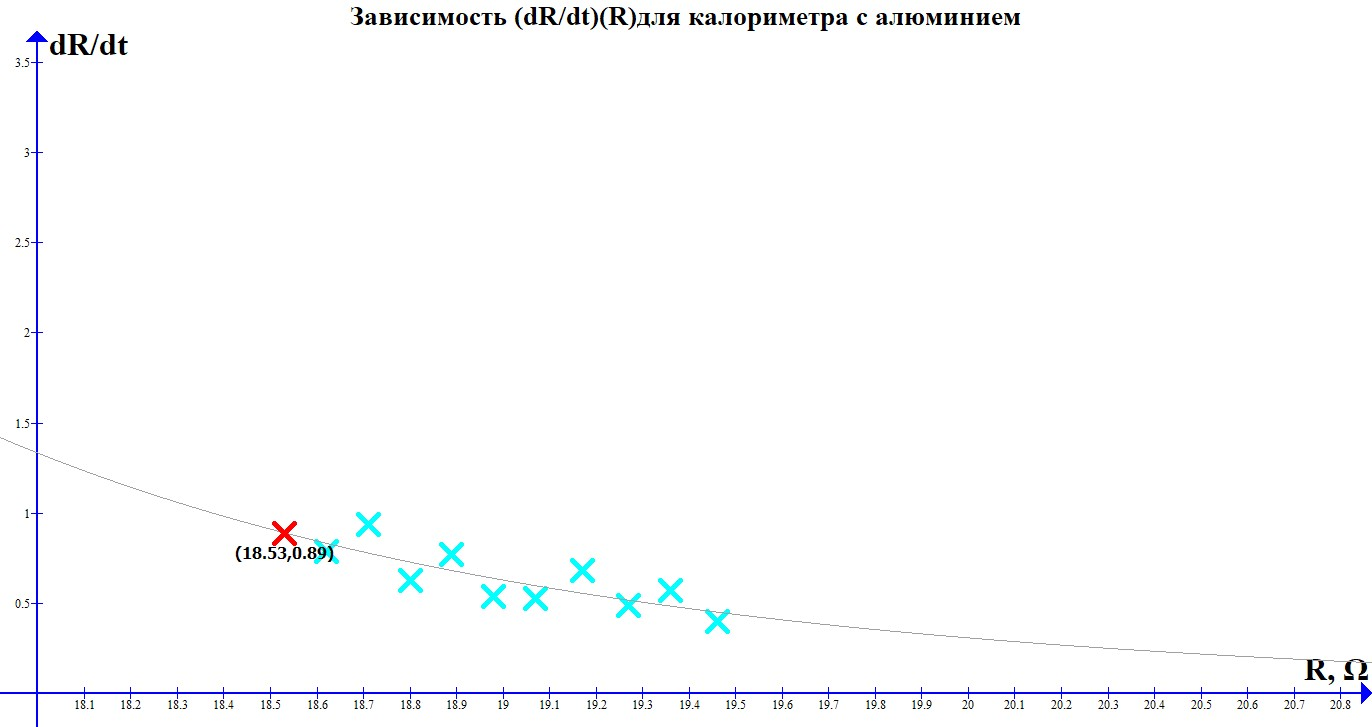
\includegraphics[scale=0.35]{2146}
\end{center}

6) Посчитаем для каждого из получнных графиков  теплоемкость по формуле: $$C=\frac{PR_k\alpha}{(dR/dt)_k(1+\alpha\Delta T_k)}$$

$C_0$=455 $\frac{Joule}{K}$

$C_1$=666 $\frac{Joule}{K}$

$C_2$=931 $\frac{Joule}{K}$

Зная, что массы тел из латуни и алюминия равны соответственно 878$\pm$0.1 g и  294.7$\pm$0.1 g  получаем их удельную теплоемкость: \\

$C_L$=240$\pm$0.3 $\frac{Joule}{K*kg}$ \hspace{40pt} $C_L$(Tabl)=377 $\frac{Joule}{K*kg}$

$C_{Al}$=1615$\pm$0.3 $\frac{Joule}{K*kg}$ \hspace{31pt} $C_{Al}$(Tabl)=897 $\frac{Joule}{K*kg}$

Также используя, что молярные массы латуни и алюминия равны $64$ и $27$ $\frac{g}{mole}$ найдем их молярную темплоемкость:\\

$C_P$(L)=15.36$\pm$0.02 $\frac{Joule}{K*mole}$ \hspace{40pt} $C_L$(Tabl)=24.128 $\frac{Joule}{K*mole}$

$C_{P}$(Al)=43.605$\pm$0.001 $\frac{Joule}{K*mole}$ \hspace{31pt} $C_{Al}$(Tabl)=24.35 $\frac{Joule}{K*mole}$











\end{document} % конец документа